\documentclass{article}

\usepackage{listings}
\usepackage{xcolor}
\usepackage{makecell}
\usepackage{graphicx}
\graphicspath{ {./resources/} }

\renewcommand\theadfont{\bfseries}


% 1’eren er sjov fordi I kan gøre lidt ala det med optimerings-opgaven, 
% dokumentere med flotte box-plots osv. Måske kan I finde en hurtigere 
% implementation, at sammenligne med.

% Emne: PriorityQueue i Java
%     Udforsk den inbyggede PriorityQueue i Java
%     Hvorfor er den ikke god? (kan ikke updatere entries, kun linære ændringer (ingen indbygget update() metode))
%     Big O notation
%     Måske en bedre måde at lave den på, eller i hvert fald ideer til forbedringer

% The Dark Side of Java's PriorityQueue
% The Missing Piece in Java's PriorityQueue
\title{Java PriorityQueue Class} 

\author{Anders Jacobsen, Dima Karaush}

% color definition (used for listings)
\definecolor{codegreen}{rgb}{0,0.6,0}
\definecolor{codegray}{rgb}{0.5,0.5,0.5}
\definecolor{codepurple}{rgb}{0.58,0,0.82}
\definecolor{backcolour}{rgb}{0.94,0.94,0.94}

% Designing our listing (Credits to Mutestock : https://github.com/Mutestock)
% He made this style and reviewed an ealier assignment and pointed out that 
% my listing could be improved.
\lstdefinestyle{mystyle}{
    backgroundcolor=\color{backcolour},   
    commentstyle=\color{codegreen},
    keywordstyle=\color{magenta},
    numberstyle=\tiny\color{codegray},
    stringstyle=\color{codepurple},
    basicstyle=\ttfamily,
    breakatwhitespace=false,         
    breaklines=true,                 
    captionpos=b,                    
    keepspaces=true,                 
    numbers=left,                    
    numbersep=5pt,                  
    showspaces=false,                
    showstringspaces=false,
    showtabs=false,                  
    tabsize=2
}

% setting the style to my listings
\lstset{style=mystyle, language=Java}

\begin{document}
\maketitle

\begin{abstract}
    Java's PriorityQueue class have a bottleneck when you need to update values in the queue.
    Depending on the use and implementation, Java's PriorityQueue can add serious performance 
    issues when accessing the data not using the poll() method.
    When updating a value in the queue, performance can be improved by more than 50\% compared 
    to Java's PriorityQueue implementation. Implementing your own version might remove this 
    bottleneck from your software. 
\end{abstract}

\section{Introduction}
This article will discuss Java's "Build-in" class \lstinline!PriorityQueue!. 
The interest for this topic has grown from an implmentation of a weighted graph 
in Java, which we found had a possible shortcomming for our use-case. The shortcomming was that to update
a value in the queue, we had to use a linear search (loop) through the queue to update 
a value within. That is fine on a small scale, but what if need to draw a graph of all the cities in the world? 
We believe that this has space for optimization and that is why this article explores this subject.  

We plan to use Peter Sestofts Mark5 benchmarking techniques from his article 
"Microbenchmarks in Java and C\#" \cite{microbenchmarks} to bencnhmark the two 
PriorityQueues. We will do seperate benchmarking with warmup iterations on 
each of the implementations. Afterwards we will explore the data using a Python
Notebook. Then we compare the results to explore our findings. 


\section{Scope}
This article aims to compare the performance between Java's PriorityQueue
and a PriorityQueue we designed and implemented. The article will only include 
perfomance comparisson for the task to update an Object within. It will not 
compare the enqueing or dequeing performance times.

\section{Problem}
\subsection{Background}
% There's no way to find an element in a heap, but to go through all the 
% elements, though pruning (Stop searching if a bigger node is reached) is possible. 
% Therefore a list will be used to make search possible
Java's PriorityQueue is build using a heap, this means that there is no way to quickly find an Object within.
Therefore it is nessesary to do a linear iteration through the queue. This is made possible by 
the iterator method inherited in the PriorityQueue class. What we want to explore is how much faster it would 
be to use fx. binary search in a sorted array representing a queue instead.  
\subsection{Problem Statement}
\begin{enumerate}
    \item How fast is Java's current implmentaion, when the task is to update a value within?
    \item How fast is our implementation of PriorityQueue using binary search to find and update a value within?
    \item How do the queues compare in performance?
\end{enumerate}


\section{Analysis}
\subsection{Benchmark Method} % Cosby
This subsection will cover how we prepared and executed our benchmarks.
It will also touch the subject of what we are timing in the two implementations
of a PriorityQueue. We've followed Peter Sestofts approach to microbenchmarking in 
Java \cite{microbenchmarks}, we've used a combination of Mark5 and Mark3 
benchmarks with a few twists here and there. 
To make benchmarks, a Timer class is nessesary. We've designed the a simplest
version possible to avoid interference from calculations in the Timer class.

\begin{lstlisting}[caption={Simple Timer class implementation},label={lst:timerclass}]
    public class Timer {
        private long start;

        public void start() {
            start = System.nanoTime();
        }

        public long step() {
            return System.nanoTime() - start;
        }
    }
\end{lstlisting}

This implementation enables us to process the times as nano seconds after 
the benchmarks and also to easily restart the timer.

In addition to the Timer class we have also implemented a TimerTracker class.
This class only consists of two lists that can contain the warmup and real 
benchmark times. Also a method for writing the optained times to a CSV\footnote{Comma Seperated Values Filestructure} file.
The CSV files will be used to explore the data later. 

\begin{lstlisting}[caption={Benchmark iterations}, label={lst:benchmarkiterations}]
    private static void benchmarkPriorityQueue(int warmupIterations, int iterations, TimeTracker tracker) {
        // Printing removed for simplicity
        // Warmup
        for (int i = 0; i < warmupIterations; i++) {
            tracker.addWarmupTime(pQueueRun());
        }
        // Benchmark
        for (int i = 0; i < iterations; i++) {
            tracker.addTime(pQueueRun());
        }
    }
\end{lstlisting}

%How do we measure the times
Measurements in the benchmark is done only on the time it takes to update 
a value in the PriorityQueue. Again we follow Peter Sestofts microbenchmarking 
techniques. In listing \ref{lst:benchmarkiterations} we run a number of warmup iterations before running the
actual benchmark. This is to fight the battle agains Java's JIT\footnote{Just In Time} 
compiler as described in Peter Sestofts article. In the listing the method 
\lstinline{pQueueRun()} is running the benchmark, this will be descriped 
in section \ref{sec:javabenchmark}. The \lstinline{tracker.addTime(long time)} 
simply adds a time to a list that will later be written to a CSV file.

%remember ref to pdf (peter sestoft i disc)
%Something about out Timer, TimerTracker class
%How do we measure the times
%What do we time (ONLY UPDATE)
%Why do we do as we do
\subsection{Benchmark of Java's priorityQueue} % Dima
\label{sec:javabenchmark}
%Describe the method for updating (LINEAR WITH ITERATOR)
To understand the example that we are using we have to take a look at how we use our \lstinline{pQueueRun()}.

\begin{lstlisting}[caption={Populating the queue},label={lst:Populating_the_queue}]
    PriorityQueue<Node> pQueue = new PriorityQueue<>(QUEUE_LENGTH, nodeComp);

    // Filling the queue with Nodes
    for (int i = 0; i < QUEUE_LENGTH; i++) {
        pQueue.add(new Node(i, i + 1, i));
    }
\end{lstlisting}

We create a simple priorityQueue that takes nodes as an object. Then we add some nodes that fill up the queue, 
the nodes do not require any special values. But we do add a unique value to each so that we are able to distinguish the nodes from each other.
% Show a desciption of our numbers
As we are running the benchmark and the times are loaded into the CSV file 5000 times. We can get can get an overview of the times that we have saved in the .CSV file.
Running the results through a python notebook, we can get a description of the data.
\begin{table}[hbt!]
\centering
\begin{tabular}{ |l|r| }
    \hline
    \thead{count}	& 5000	                   \\
    \thead{mean}	& 1046789.700000 ns        \\ 
    \thead{std}	    & 116796.066013 ns	       \\
    \thead{min}	    & 844800.000000	ns         \\
    \thead{25\%}	& 973000.000000	ns         \\
    \thead{50\%}	& 1030100.000000 ns        \\
    \thead{75\%}	& 1097700.000000 ns        \\
    \thead{max}	    & 2193600.000000 ns        \\
    \hline
\end{tabular}
    \caption{Key numbers from benchmark} 
    \label{tab:regular_times}
\end{table}


\paragraph{Mean and standard deviation}
Looking at the mean we can se the that the average time for an update is about 1/1000 th of a second. 
And the standard devisation is at about +/- 1/10000th of that.

Here we have zoomed in on a boxplot of the data.

\begin{figure}[hbt!]
\label{img:boxplotorg}
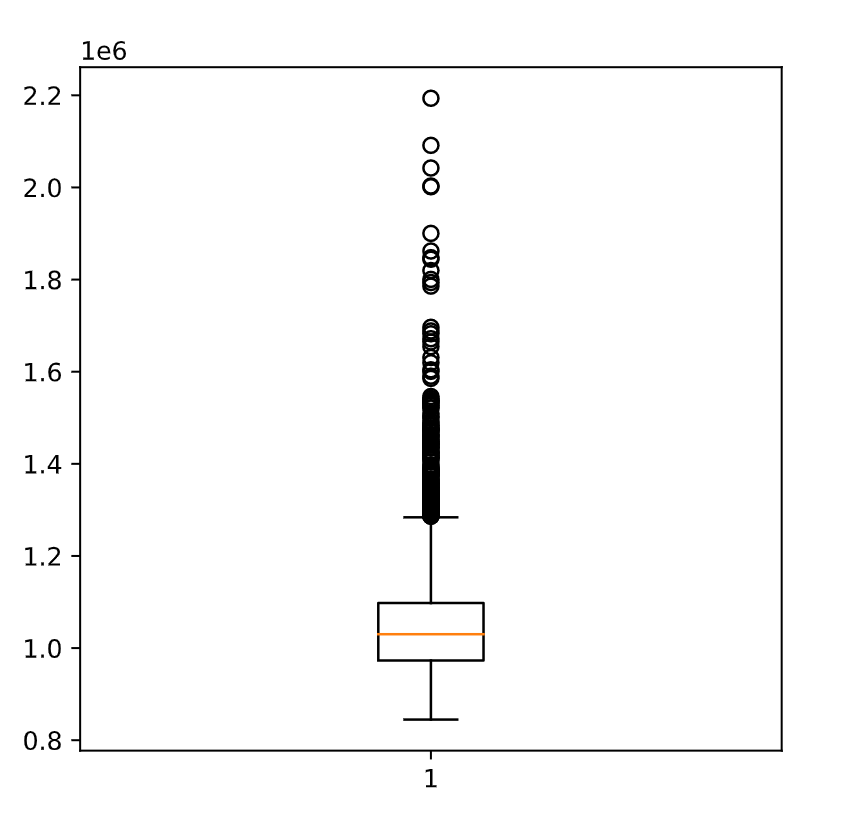
\includegraphics[width=\textwidth]{boxplotorg}
\caption{Benchmark boxplot}
\end{figure}


% Show boxplot of times
\subsection{Update Method} % Dima
When we are looking at updating a node in Java's priority queue. There is no method to retrieve a specific node from the list.
That is why we use an Iterator to list through every node in our list until we find a match.

\begin{lstlisting}[caption={Finding the node},label={lst:Finding_the_node}]
    Iterator<Node> it = pQueue.iterator();

    timer.start();
    while (it.hasNext()) {
        n = it.next();
        if (count == QUEUE_LENGTH - 1) {
            n.verticeTo = 80085;
            time = timer.step();
            break;
        }
        count++;
    }
\end{lstlisting}

Notice that we are listing through the queue in a linear way, which is not the most efficient way of searching through a list. 
The worst case scenario in a linear search is that our node has the highest weight and thus ends in the end of the list. 
This is also the scenario that we simulate, by updating the node when the check in the code: Listing \ref{lst:Finding_the_node} "\lstinline{if (count == QUEUE_LENGTH - 1)}" is true.

% Descripe how we implemented our search 
% Descripe that we are NOT using a heap and maybe that our 
% PriorityQueue is MUCH slower than java, in everything but the update method
\subsection{Benchmark of updateable PriorityQueue} % Cosby
% Describe the method for updating (LINEAR WITH ITERATOR)
The way we benchmarked our implmentation of the PriorityQueue can be seen on listing \ref{lst:benchmark_of_selfpq}.

\begin{lstlisting}[caption={Benchmark implmentation on our PriorityQueue},label={lst:benchmark_of_selfpq}]
    private static long pQueueRun() {
        // Initialization removed for simplicity

        timer.start();
        Node n = queue.retrieve(new Node(500, 1000, QUEUE_LENGTH-1));
        n.verticeTo = 101;
        time = timer.step();

        return time;
    }
\end{lstlisting}

As seen on the listing we have removed the initializing for simplicity in the exapmle. 
So keep in mind that a new queue and timer are initialized every iteration before the benchmark. 
In the example its visible that we use our \lstinline{retrieve()} method to get a specific 
node from the queue. We then mutate a value on the node, and stop the timer. 
Afterwards the time is returned. Later in the benchmark, the returned time is being saved in the
\lstinline{TimerTracker} witch writes it to a CSV file. 

We have explored the data from the CSV file using a Python Notebook. This gave us the 
results that can be found on table \ref{tab:updated_times}. Be aware that the times are measured in nano seconds. 

% [hbt!] for placing the table "right here" in the document 
% and not float at bottom or top of the page
\begin{table}%[hbt!] 
    \centering
    \begin{tabular}{|l|r|}
        \hline
        \thead[l]{Count}        & 5000     \\ 
        \thead[l]{Mean}         & 409.860000 ns \\  
        \thead[l]{Std. Dev.}    & 754.987935 ns \\
        \thead[l]{Min}          & 100.000000 ns \\
        \thead[l]{25\%}         & 300.000000 ns \\
        \thead[l]{50\%}         & 300.000000 ns \\ 
        \thead[l]{75\%}         & 400.000000 ns \\
        \thead[l]{Max}          & 31800.000000 ns \\
        \hline
    \end{tabular}
    \caption{Key numbers from updated benchmark} 
    \label{tab:updated_times}
\end{table}

When considering a standard deviation of 754.987935 ns and a mean of 409.86 ns on table \ref{tab:updated_times}.
We can see that we get much faster and more stable results from the updated algoritm. In the section
\ref{sec:comparisson_of_priorityqueues} we will
visualize these numbers as boxplots and compare the results.


% Show a desciption of our numbers
% Show boxplot of times
\subsection{Comparisson of PriorityQueues} % Dima
\label{sec:comparisson_of_priorityqueues}
% How much faster is the method than Javas
% Boxplots with comparrison
\begin{figure}[h]
\label{img:boxplot_comparisson}
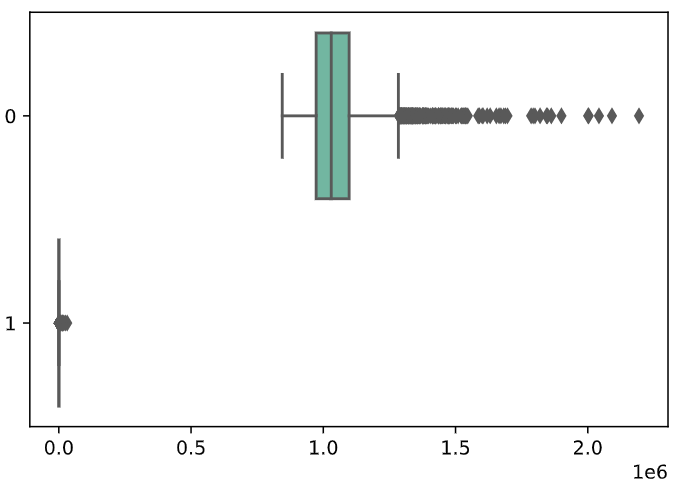
\includegraphics[width=\textwidth]{boxplot_comparisson}
\caption{Comparisson of the the Priorityqueues}
\end{figure}


\section{Conclusion} % Cosby
Answer our questions and possibly introduction
% Something about how much faster our queue is at updating
Updating a value already placed in the queue in Java's PriorityQueue is relatively
fast. With a median of 1.0301 ms searching for a node in a queue with a length of 
500000. But our implementation is comming in much fast at 300 ns, that is a 99.97\% 
increase in performance. We are not sure if these numbers are precise, since we havn't 
tested it on various machines, only one. 

% Something about how our results are to be taken with a grain of salt, 
% since our priority queue inserts elements linear, therefore it's much 
% slower at everything else in Java's PriorityQueue. 

\bibliographystyle{unsrt}
\bibliography{references}

\end{document}

% \item How fast is Java's current implmentaion, when the task is to update a value within?
% \item How fast is our implementation of PriorityQueue using binary search to find and update a value within?
% \item How do the queues compare in performance?